\documentclass{article}
\usepackage[utf8]{inputenc}

\usepackage{tikz}
\usetikzlibrary{positioning}

\begin{document}

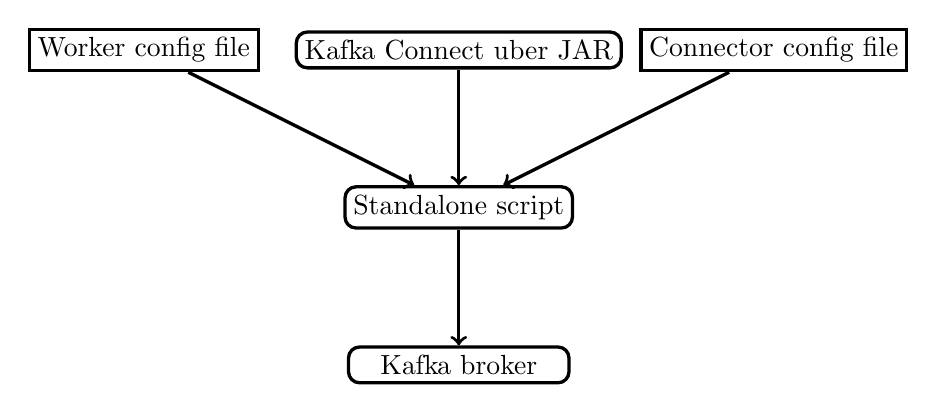
\begin{tikzpicture}[ % has a lot of options; consult the pgf manual
bend angle=45,
square/.style={rectangle, draw=black, fill=white, very thick, inner sep=3pt, minimum width=28mm},
rounded_square/.style={rectangle, rounded corners, draw=black, fill=white, very thick, inner sep=3pt, minimum width=28mm},
both_arrow/.style={<->, very thick},
out_arrow/.style={->, very thick},
in_arrow/.style={<-, very thick},
above_edge_text/.style={above, midway, sloped}
]



\node[square](worker_config) at (0,0) {Worker config file};
\node[rounded_square](connect) at (4,0) {Kafka Connect uber JAR};
\node[square](connector_config) at (8,0) {Connector config file};

\node[rounded_square](standalone) at (4,-2) {Standalone script};

\node[rounded_square](kafka_broker) at (4,-4) {Kafka broker};



\draw[out_arrow](worker_config) to [] node[auto,swap]{} (standalone);
\draw[out_arrow](connect) to [] node[auto,swap]{} (standalone);
\draw[out_arrow](connector_config) to [] node[auto,swap]{} (standalone);

\draw[out_arrow](standalone) to [] node[auto,swap]{} (kafka_broker);
\end{tikzpicture}

\end{document}